\documentclass[xcolor={usenames,dvipsnames,svgnames}, compress]{beamer}

% \usepackage[utf8]{inputenc}
\usepackage{booktabs}
\usepackage{dcolumn}
\usepackage{colortbl}
\usepackage{hyperref}
\usepackage[no-math]{fontspec}
\usepackage{ifxetex}
\usepackage{amsmath}
\usepackage{biblatex}


\usetheme{enziteto}


\begin{document}

% \title{Metodi di Apprendimento Statistico-Relazionale: Sum-Product Network \& Co-clustering}
\title{Iterated Pysoner Dilemma}
\subtitle{Or how altruistic behaviour can emerge by iterating selfish games}
\author{Antonio Vergari}
% \institute{Lacam$@$DIB$@$Uniba}
\institute{Università degli Studi di Bari}
\department{Dipartimento di Informatica}
\laboratory{LACAM}
\group{Machine Learning}
\institutelogo{
\includegraphics[width=25pt]{figures/unibaba}}
\lablogo{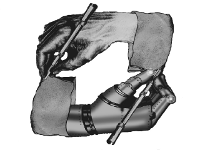
\includegraphics[width=35pt]{figures/lacam}}

{
  \setbeamertemplate{headline}{}
  \setbeamertemplate{footline}{}
  \begin{frame}
    \titlepage
  \end{frame}
}

\end{document}

%%% Local Variables:
%%% mode: latex
%%% TeX-master: t
%%% TeX-engine: xetex
%%% End:
